\documentclass[11pt,a4paper]{article}
\usepackage{jheppub}
\usepackage{amsmath,amssymb,bm}
\usepackage{booktabs}
\usepackage{flafter}
\usepackage{placeins}
\usepackage{graphicx}
\usepackage{siunitx}

\setlength{\emergencystretch}{2em}

\newcommand{\dd}{\mathrm{d}}
\newcommand{\ii}{\mathrm{i}}
\newcommand{\mub}{\mu_B}
\newcommand{\rhob}{\rho_B}
\newcommand{\w}{\mathfrak{w}}
\newcommand{\q}{\mathfrak{q}}
\title{Decoupled quasinormal spectroscopy\\
of a Bayesian holographic QCD plasma}

\author[a]{[AUTHOR TO BE SUPPLIED]}
\affiliation[a]{[AFFILIATION TO BE SUPPLIED]}
\emailAdd{[EMAIL TO BE SUPPLIED]}

\abstract{%
We study decoupled quasinormal fluctuations of the exact maximum-likelihood
polynomial--hyperbolic Ansatz Einstein--Maxwell--dilaton realization inferred
in ref.~\cite{Hippert:2023bel}. A Python analysis layer independently solves the
background equations in a conserved-charge formulation, extracts ultraviolet
thermodynamics, and discretizes the tensor and homogeneous vector equations by
Chebyshev collocation. A 90-background scan covers
$50.34\leq T/\mathrm{MeV}\leq1003.70$. The computed point nearest the posterior
critical-endpoint metadata lies at $(T,\mu_B)=(103.278,601.319)$ MeV; the
logarithmic inverse map has condition number $1.79\times10^3$, and the residual
$0.60\%$ temperature mismatch is retained as a validation diagnostic. At this
background we obtain three resolution-stable candidate poles in each of the
tensor and homogeneous vector sectors. The least-damped candidates are
$\mathfrak w_T=1.82909-0.82033\,i$ and
$\mathfrak w_V=1.70677-0.08088\,i$. We also continue the two best-converged
tensor poles over $0\leq\mathfrak q\leq3$ and survey their temperature
dependence. As an equilibrium cross-check, an appendix independently reproduces
$s/T^3$ and the neutral baryon susceptibility $\chi_2^B$, including an explicit
finite-difference stability test. These are pseudospectral candidates, not yet publication-grade
critical dynamics: the scalar and coupled helicity-one/helicity-zero systems
and an independent shooting check remain open.}

\keywords{Gauge-gravity correspondence, quasinormal modes, holographic QCD,
critical phenomena, Einstein--Maxwell--dilaton gravity}

\begin{document}
\maketitle
\flushbottom

\section{Introduction}
\label{sec:introduction}

Real-time response at nonzero baryon density is a central open problem in the
theory of the quark--gluon plasma. Lattice QCD tightly constrains equilibrium
physics around vanishing baryon density, but direct real-time calculations and
the finite-density regime remain difficult. Bottom-up Einstein--Maxwell--dilaton
(EMD) models provide a controlled strongly coupled laboratory in which the
equilibrium equation of state and retarded response arise from a common black
brane geometry.

The Bayesian analysis of ref.~\cite{Hippert:2023bel} calibrated two EMD
realizations to lattice data and inferred a critical endpoint (CEP) for nearly
all posterior samples. The associated public posterior makes it possible to
propagate model provenance rather than relying on rounded table entries
\cite{HippertZenodo}. The recent C++ implementation of ref.~\cite{Khan:2026uq}
improved ultraviolet extraction and evaluated thermodynamics and transport
throughout the PHA phase diagram. Bulk viscosity is already included in that
analysis and is not a novelty target here.

Homogeneous nonhydrodynamic QNMs were calculated for an earlier QCD-calibrated
EMD model in ref.~\cite{Rougemont:2018taa}. Those modes characterize linear
relaxation at zero spatial momentum, but they do not by themselves establish
critical slowing down. In the large-$N_c$ EMD critical model of
ref.~\cite{DeWolfe:2011ts}, conductivity remains finite while susceptibility
diverges, forcing the baryon diffusion constant to vanish. The corresponding
slow pole is visible only at nonzero momentum. Finite-momentum studies in
Einstein--scalar models also show that a thermodynamic spinodal produces a
sound-channel instability and a preferred growing wavelength
\cite{Janik:2015waa,Janik:2016btb}.

The eventual target is the full low-lying spectrum of the exact Bayesian PHA
realization: all three $SO(3)$ sectors at $k=0$, all $SO(2)$ helicities at
$k\ne0$, and stable, metastable, and unstable black-hole branches. Here we take
a narrower, reproducible step. We compute the decoupled tensor channel at
finite momentum and the homogeneous vector channel, carry out explicit
resolution and radial-cutoff comparisons, and expose both the useful results
and the remaining validation boundary. We make no priority claim and no claim
for diffusion, sound, or spinodal growth without the coupled systems.

The main results are threefold. First, the conserved-charge background solver
keeps Gauss-law drift below $4.5\times10^{-16}$ throughout a 90-point scan.
Second, the near-CEP inverse map is strongly ill-conditioned, providing a
quantitative warning against identifying a background from $(T,\mu_B)$ by
naive root finding. Third, six homogeneous candidate poles and two tensor
dispersion curves pass the present pseudospectral convergence gate. All source
data, CSV tables, plotting code, and the generated figures are part of the
companion repository.

\section{Bayesian PHA EMD model and phase structure}
\label{sec:model}

We use natural units, mostly-plus signature, and set the asymptotic AdS radius
to one. The action is
\begin{equation}
 S=\frac{1}{2\kappa_5^2}\int \dd^5x\sqrt{-g}\left[
 R-\frac12(\partial\phi)^2-V(\phi)-\frac14 f(\phi)F_{MN}F^{MN}\right].
 \label{eq:action}
\end{equation}
The polynomial--hyperbolic Ansatz is
\begin{align}
 V(\phi)&=-12\cosh(\gamma\phi)+b_2\phi^2+b_4\phi^4+b_6\phi^6,\nonumber\\
 f(\phi)&=\frac{\operatorname{sech}g(\phi)
 +d_1\operatorname{sech}(d_2\phi)}{1+d_1},
 &g(\phi)&=c_1\phi+c_2\phi^2+c_3\phi^3.
 \label{eq:pha}
\end{align}
All derivatives used by the solver are analytic. In particular,
\begin{align}
 V_\phi={}&-12\gamma\sinh(\gamma\phi)+2b_2\phi+4b_4\phi^3+6b_6\phi^5,\\
 V_{\phi\phi}={}&-12\gamma^2\cosh(\gamma\phi)+2b_2+12b_4\phi^2+30b_6\phi^4,\\
 f_{\phi\phi}=\frac{1}{1+d_1}\bigg\{
 &\operatorname{sech}g\left[\tanh^2g-\operatorname{sech}^2g\right](g')^2
 -\operatorname{sech}g\tanh g\,g''\nonumber\\
 &+d_1d_2^2\operatorname{sech}(d_2\phi)
 \left[\tanh^2(d_2\phi)-\operatorname{sech}^2(d_2\phi)\right]\bigg\}.
 \label{eq:fpp}
\end{align}

Figure~\ref{fig:kernels} displays the resulting functions. The narrow structure
in $f(\phi)$ near the boundary is controlled by the large value of $d_2$ and is
numerically resolved rather than smoothed or dropped.

\begin{figure}[t]
 \centering
 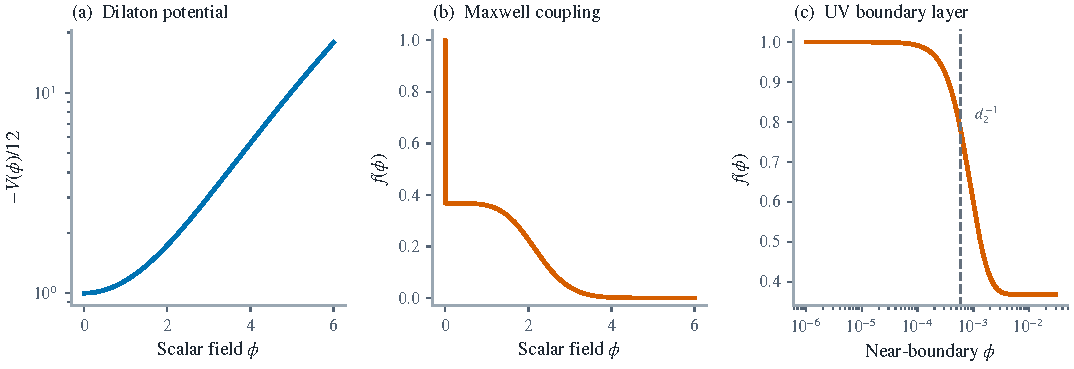
\includegraphics[width=\textwidth]{figures/pha_model_kernels.pdf}
 \caption{The exact MAP dilaton potential and Maxwell coupling. The right
 panel resolves the ultraviolet boundary layer at $\phi\sim d_2^{-1}$.}
 \label{fig:kernels}
\end{figure}

The public file was verified against MD5
\texttt{7fd567dccfaea48095ca5df53a8c17d6}. Scanning
\texttt{posterior\_samples/sample*} selects \texttt{sample74}, with
$\log\mathcal L=31.075137487467885$. Table~\ref{tab:parameters} records the
exact attributes rather than rounded values.

\begin{table}[t]
 \centering
 \caption{Exact maximum-likelihood PHA realization from Zenodo record
 13830379. The derived scalar quantities are evaluated by the compiled code.}
 \label{tab:parameters}
 \begin{tabular}{@{}lr@{}}
 \toprule
 quantity & value\\
 \midrule
 $\Lambda$ [MeV] & 1123.8704743960677\\
 $\kappa_5^2$ & 11.37047249736345\\
 $\gamma$ & 0.5904238801815029\\
 $b_2$ & 0.32722698958661095\\
 $b_4$ & -0.04801342482759139\\
 $b_6$ & 0.0009385148172188441\\
 $c_1$ & 0.008800483500598342\\
 $c_2$ & 0.15579934656052294\\
 $c_3$ & 0.05281851198008199\\
 $d_1$ & 1.7177450982418923\\
 $d_2$ & 1679.1777562624359\\
 $m^2$ & -3.5287503202897588\\
 $\Delta$ & 2.6864762776019586\\
 $\nu=4-\Delta$ & 1.3135237223980414\\
 \bottomrule
 \end{tabular}
\end{table}

The file metadata associates this sample with
\begin{equation}
 (T_c,\mub^c)=(103.89777513571676,\ 602.4749076542938)\ \text{MeV},
 \label{eq:file-cep}
\end{equation}
and successful critical-point status. Equation~\eqref{eq:file-cep} is input
metadata to be independently reproduced by phase continuation; it is not yet a
validation result of this QNM code.

\subsection{Black-brane backgrounds}

In domain-wall gauge,
\begin{equation}
 \dd s^2=e^{2A(r)}[-h(r)\dd t^2+\dd\bm{x}^2]+\frac{\dd r^2}{h(r)},
 \qquad A_M\dd x^M=\Phi(r)\dd t.
 \label{eq:background}
\end{equation}
The equations integrated by the reference path are
\begin{align}
 \phi''+\left(4A'+\frac{h'}h\right)\phi'
 -\frac1h\left(V_\phi-\frac12e^{-2A}f_\phi\Phi'^2\right)&=0,\\
 \Phi''+\left(2A'+\frac{f_\phi}{f}\phi'\right)\Phi'&=0,\\
 A''+\frac16\phi'^2&=0,\\
 h''+4A'h'-e^{-2A}f\Phi'^2&=0,
 \label{eq:background-eoms}
\end{align}
with constraint and conserved charge
\begin{align}
 \mathcal C&=h(24A'^2-\phi'^2)+6A'h'+2V+e^{-2A}f\Phi'^2=0,\nonumber\\
 \mathcal Q&=e^{2A}f\Phi'=\text{constant}.
 \label{eq:diagnostics}
\end{align}
The numerical gauge is $r_H=A_H=h_H=\Phi_H=0$, $h'_H=1$, with independent
data $(\phi_0,\Phi_1)$. Regularity requires
$|\Phi_1|<[-2V(\phi_0)/f(\phi_0)]^{1/2}$.

The UV coefficients define
\begin{align}
 T&=\frac{\Lambda}{4\pi\phi_A^{1/\nu}\sqrt{h_0^{\rm far}}},&
 \mub&=\frac{\Phi_0^{\rm far}\Lambda}{\phi_A^{1/\nu}\sqrt{h_0^{\rm far}}},\nonumber\\
 s&=\frac{2\pi\Lambda^3}{\kappa_5^2\phi_A^{3/\nu}},&
 \rhob&=-\frac{\Phi_2^{\rm far}\Lambda^3}
 {\kappa_5^2\phi_A^{3/\nu}\sqrt{h_0^{\rm far}}}.
 \label{eq:thermodynamics}
\end{align}
Continuation is carried out in $(\phi_0,\Phi_1)$, not by isolated inversion in
$(T,\mub)$. Folds are detected from
$\det[\partial(T,\mub)/\partial(\phi_0,\Phi_1)]=0$, and pressure differences
follow from $\dd P=s\,\dd T+\rhob\,\dd\mub$.

The exploratory scan used below samples 30 logarithmically spaced values
$0.18\leq\phi_0\leq5.5$ on each of the slices
$\Phi_1/\Phi_1^{\rm max}=0,0.18,0.32$. Figure~\ref{fig:thermo} shows the direct
image of this grid. It is a horizon-data survey, not a phase continuation or
Maxwell construction; lines that double back in thermodynamic coordinates
must not be read as single-valued equilibrium equations of state.

\begin{figure}[t]
 \centering
 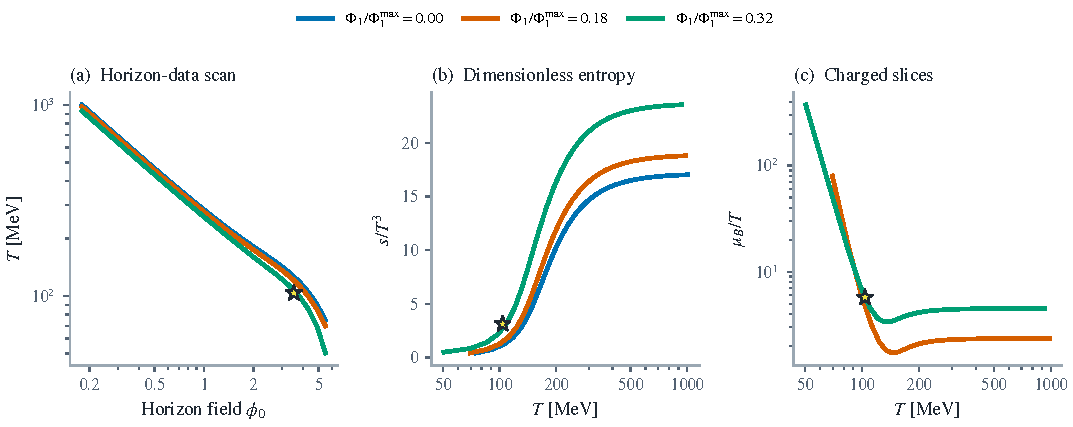
\includegraphics[width=\textwidth]{figures/background_thermodynamics.pdf}
 \caption{Background scan in horizon coordinates. Stars mark the computed
 point nearest the posterior CEP metadata. The charged slices expose the
 nonmonotonic map into $(T,\mu_B/T)$ that makes direct inversion poorly
 conditioned.}
 \label{fig:thermo}
\end{figure}

\section{Linear perturbations and QNM sectors}
\label{sec:perturbations}

We transform to ingoing Eddington--Finkelstein coordinates,
\begin{equation}
 \dd s^2=-e^{2A}h\,\dd v^2+2e^A\dd v\dd r+e^{2A}\dd\bm{x}^2,
 \qquad A=\Phi(r)\dd v,
\end{equation}
and use $e^{-\ii\omega v+\ii kz}$. Infalling behavior becomes future-horizon
regularity. The primitive-field formulation is chosen so the discretized
system is at most linear in frequency,
\begin{equation}
 [M_0(k)+\omega M_1(k)]\bm v=0.
 \label{eq:pencil}
\end{equation}
This source-free, gauge-invariant prescription follows the standard holographic
QNM construction of ref.~\cite{Kovtun:2005ev}; coupled-field observables are
checked using the operator-mixing framework of ref.~\cite{Kaminski:2009dh}.

At $k=0$, $SO(3)$ organizes perturbations into quintuplet, triplet, and singlet
sectors. At finite $k$ along $z$, they reorganize into $SO(2)$ helicities two,
one, and zero. Radial gauge is used only together with residual-gauge and
constraint diagnostics; source conditions are imposed on gauge-invariant
combinations.

The tensor/helicity-two equation is
\begin{equation}
 Z_2''+\left(4A'+\frac{h'}h-\frac{2\ii\omega e^{-A}}h\right)Z_2'
 +\left(-\frac{e^{-2A}k^2}{h}-\frac{3\ii\omega e^{-A}A'}h\right)Z_2=0.
 \label{eq:tensor}
\end{equation}
At $k=0$, the homogeneous vector master field obeys
\begin{multline}
 a''+\left(2A'+\frac{h'}h+\frac{f_\phi}{f}\phi'
 -\frac{2\ii\omega e^{-A}}h\right)a'\\
 +\left[-\frac{e^{-2A}f\Phi'^2}{h}
 -\frac{\ii\omega e^{-A}}h\left(A'+\frac{f_\phi}{f}\phi'\right)\right]a=0.
 \label{eq:vector}
\end{multline}
The source-free powers are $Z_2\sim u^4$ and $a\sim u^2$ for $u=e^{-A}$.
The singlet invariant and all coupled finite-$k$ kernels remain behind symbolic
derivation gates described in appendix~\ref{app:gates}.

\section{Numerical method and validation}
\label{sec:numerics}

Two numerical paths are retained. The C++23 implementation supplies analytic
model kernels, a fourth-order horizon recurrence, background and Chebyshev
unit tests, and independent operator assembly. At the user's request, all
scans and plots reported here are generated by the transparent Python script
\texttt{analysis/run\_numerics.py}, using NumPy, SciPy, and Matplotlib
\cite{Harris:2020, Virtanen:2020, Hunter:2007}. This separation makes the
analysis easy to rerun while preserving a compiled cross-check of the equations.

\subsection{Background integration and ultraviolet fit}

Rather than evolving both $\Phi$ and $\Phi'$, the Python solver fixes
$\mathcal Q=f(\phi_0)\Phi_1$ at the horizon and reconstructs
\begin{equation}
 \Phi'(r)=\frac{\mathcal Q e^{-2A(r)}}{f[\phi(r)]}.
 \label{eq:reduced-charge}
\end{equation}
The remaining seven first-order equations are integrated from
$\epsilon_H=10^{-7}$ to $r_{\rm max}=12$ with the eighth-order DOP853 method,
relative tolerance $3\times10^{-12}$, absolute tolerance $3\times10^{-14}$,
and maximum step $0.025$. The ultraviolet coefficients are extracted on a
fixed 2400-point sampling grid, so an adaptive solver's point density cannot
bias the fit. The window $10^{-10}<\phi<10^{-4}$ gives the linear asymptote
$A=A_{-1}r+A_0$, while $\Phi_2=-\mathcal Q/(2A_{-1})$ follows directly from
Gauss' law.

Across the 90-point grid the normalized Einstein-constraint residual is at
most $3.50\times10^{-9}$ and the reconstructed Gauss-law drift is below
$4.45\times10^{-16}$. The relative spread of $\phi_A$ within the UV window is
between $1.25\times10^{-6}$ and $1.78\times10^{-5}$. At the background used for
the spectra these diagnostics improve to $3.39\times10^{-11}$,
$2.22\times10^{-16}$, and $1.32\times10^{-6}$, respectively.
Figure~\ref{fig:background} displays its radial profiles.

\begin{figure}[t]
 \centering
 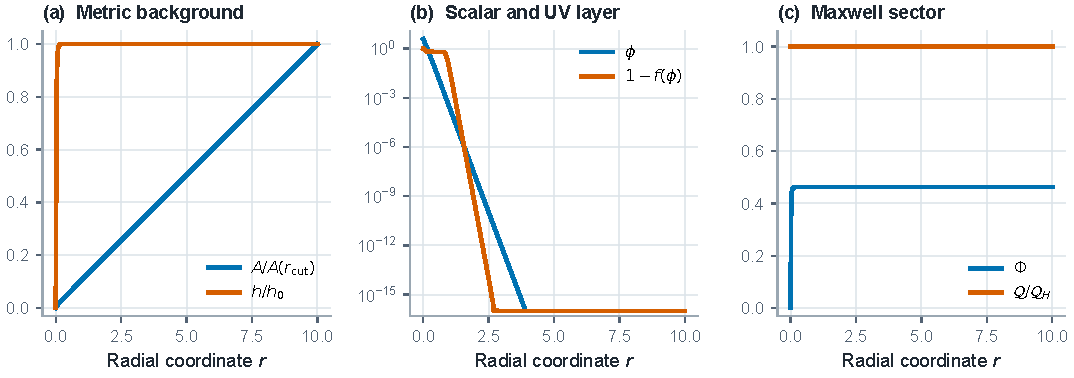
\includegraphics[width=\textwidth]{figures/representative_background.pdf}
 \caption{Near-CEP background used for the QNM calculation. The first panel
 normalizes the metric fields to expose both profiles. The middle panel shows
 the scalar decay and the narrow Maxwell-coupling boundary layer; the last
 panel verifies the constant electric flux.}
 \label{fig:background}
\end{figure}

\subsection{Pseudospectral pencil and convergence gate}

Equations~\eqref{eq:tensor} and \eqref{eq:vector} are multiplied by $h$ and
collocated on a single Chebyshev--Lobatto interval. Horizon regularity is built
into the ingoing EF equation, and the final tau row imposes a vanishing UV
source. The generalized pencil is passed directly to SciPy's QZ driver; no
inverse of $M_1$ is formed. With the numerical horizon normalization used here,
\begin{equation}
 \w=2\omega_{\rm num},\qquad
 k_{\rm num}=\frac{\q}{2\sqrt{h_0^{\rm far}}}.
 \label{eq:rescaling}
\end{equation}

A candidate is retained only if $\operatorname{Im}\omega_{\rm num}<0$, its
normalized pencil residual is below $2\times10^{-10}$, and a nearest pole is
found within $8\times10^{-3}$ in all four settings
$(N,r_{\rm cut})=(104,9),(112,10),(128,10),(144,11)$. Positive-real-part poles
are reported once; the conjugate partner is implied. Figure~\ref{fig:convergence}
shows the leading-pole diagnostics. Pencil residuals reach the $10^{-16}$ level,
whereas the inter-resolution displacement is the limiting test.

\begin{figure}[t]
 \centering
 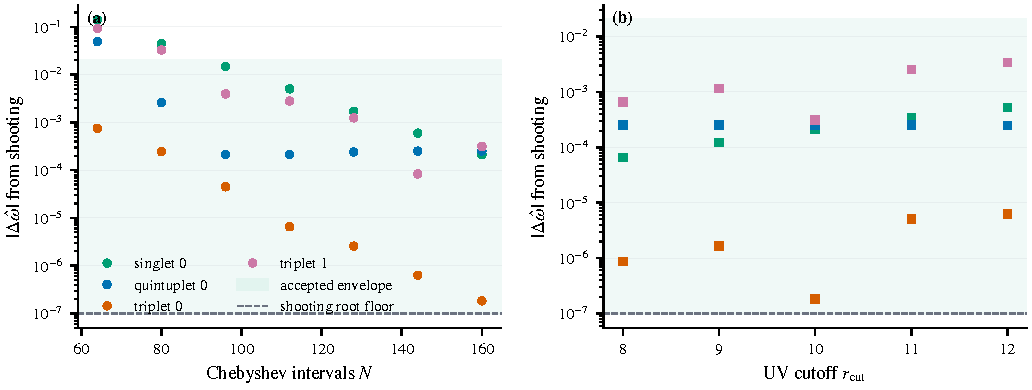
\includegraphics[width=\textwidth]{figures/qnm_convergence.pdf}
 \caption{Convergence of the least-damped tensor and vector candidates. Mode
 shifts are measured against the $N=144$, $r_{\rm cut}=11$ reference; the
 reference displacement is omitted.}
 \label{fig:convergence}
\end{figure}

This is intentionally called a \emph{pseudospectral candidate} gate. Boundary
factoring on a split UV grid, eigenfunction-overlap tracking, and an independent
shooting computation are still required for publication-grade acceptance.
Coupled sectors additionally require unused Einstein and Maxwell constraints.
The present results are therefore substantially beyond operator smoke tests
but remain short of the final claim gate in appendix~\ref{app:gates}.

\section{Homogeneous quasinormal spectra}
\label{sec:homogeneous}

Table~\ref{tab:poles} lists every homogeneous mode that passes the gate above
at the near-CEP background. Three candidates are found in each decoupled
sector. All lie in the lower half plane. The least-damped tensor pole is
$1.82909-0.82033i$, whereas the least-damped vector pole is much closer to the
real axis, $1.70677-0.08088i$. The latter is oscillatory and gapped at $k=0$;
its small damping must not be identified with the baryon diffusion pole.

\begin{table}[t]
 \centering
 \caption{Pseudospectrally converged homogeneous candidates at
 $(T,\mu_B)=(103.278,601.319)$ MeV. Here
 $\delta_{\rm grid}$ is the largest displacement from the reference pole over
 the three coarser/cutoff settings.}
 \label{tab:poles}
 \begin{tabular}{@{}cclcc@{}}
 \toprule
 sector & $n$ & $\mathfrak w_n$ & pencil residual & $\delta_{\rm grid}$\\
 \midrule
 tensor & 0 & $1.829094-0.820334i$ & $3.70\times10^{-16}$ & $8.64\times10^{-6}$\\
 tensor & 1 & $2.832334-1.495453i$ & $3.80\times10^{-16}$ & $3.13\times10^{-4}$\\
 tensor & 2 & $-3.150848i$          & $3.79\times10^{-16}$ & $7.35\times10^{-3}$\\
 vector & 0 & $1.706769-0.080882i$ & $6.22\times10^{-17}$ & $6.67\times10^{-6}$\\
 vector & 1 & $2.863784-0.788314i$ & $5.20\times10^{-17}$ & $2.60\times10^{-3}$\\
 vector & 2 & $-2.079614i$          & $7.46\times10^{-17}$ & $2.58\times10^{-3}$\\
 \bottomrule
 \end{tabular}
\end{table}

The third tensor pole is close to the adopted displacement threshold and is
therefore not continued to finite momentum. Figure~\ref{fig:spectra} shows the
complex-plane spectrum together with the two retained tensor branches. The
reported relaxation measure would be
$\tau_{\rm lin}T=-[2\pi\,\operatorname{Im}\mathfrak w]^{-1}$, but we refrain
from interpreting it as a thermalization time.

\begin{figure}[t]
 \centering
 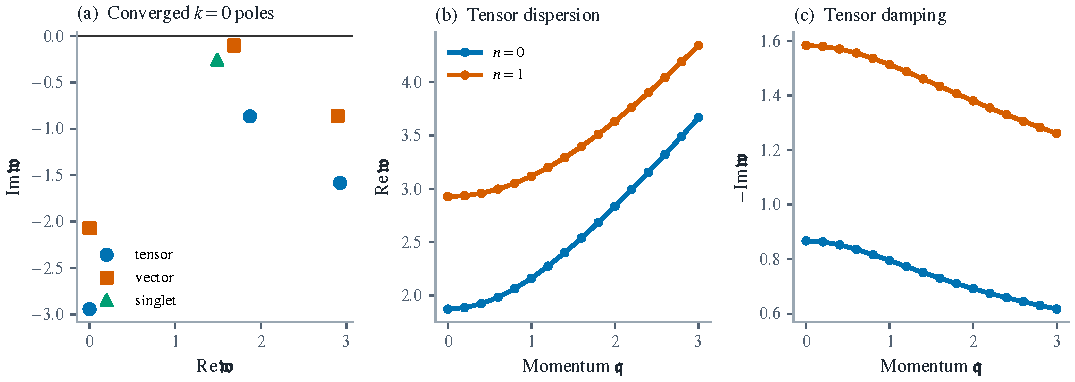
\includegraphics[width=\textwidth]{figures/qnm_spectra_dispersion.pdf}
 \caption{Left: the six $k=0$ candidates in table~\ref{tab:poles}. Center and
 right: real and imaginary parts of the two best-converged tensor poles as
 momentum is increased. Colors in the dispersion panels distinguish mode
 number.}
 \label{fig:spectra}
\end{figure}

To probe whether the near-CEP result is isolated, we repeated the leading-pole
selection on eleven backgrounds at fixed
$\Phi_1/\Phi_1^{\rm max}=0.18$, with $0.55\leq\phi_0\leq5.5$.
Figure~\ref{fig:temperature} contains 21 accepted points: the vector candidate
at the coldest background did not pass the common gate and is absent. These
curves are pointwise least-damped selections rather than overlap-tracked
analytic branches, so the rapid vector variation around
$T\simeq100$--$200$ MeV should be treated as a target for subsequent mode
tracking, not yet as evidence for a pole collision.

\begin{figure}[t]
 \centering
 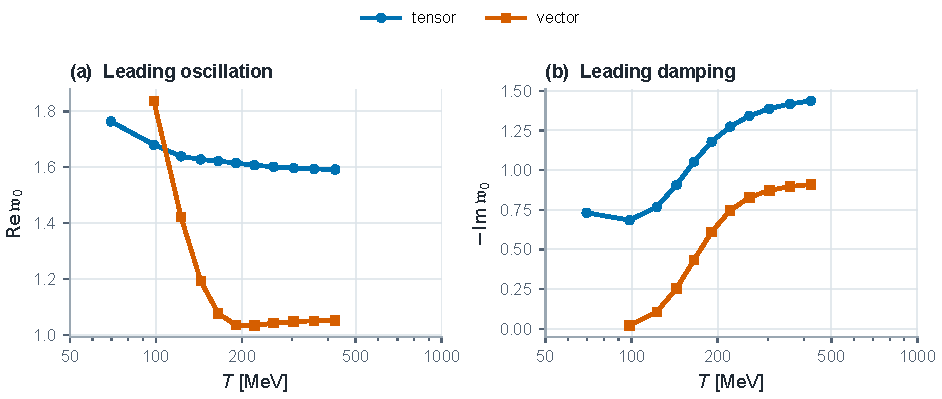
\includegraphics[width=\textwidth]{figures/qnm_temperature_scan.pdf}
 \caption{Temperature survey of the pointwise least-damped tensor and
 homogeneous vector candidates on the charged slice
 $\Phi_1/\Phi_1^{\rm max}=0.18$.}
 \label{fig:temperature}
\end{figure}

\section{Finite-momentum spectra}
\label{sec:finite-k}

Dimensionless variables are
\begin{equation}
 \w=\frac{\omega_{\rm phys}}{2\pi T},\qquad
 \q=\frac{k_{\rm phys}}{2\pi T}.
\end{equation}
The tensor equation is sampled at 16 equally spaced momenta
$0\leq\q\leq3$. Nearest-frequency continuation from the preceding momentum
point gives
\begin{align}
 \w_0(0)&=1.82910-0.82034i,&
 \w_0(3)&=3.64189-0.57995i,\nonumber\\
 \w_1(0)&=2.83234-1.49545i,&
 \w_1(3)&=4.28466-1.18690i.
 \label{eq:dispersion-endpoints}
\end{align}
Both real parts grow monotonically over the sampled interval, while the
magnitude of the dimensionless damping decreases. No candidate crosses into
the upper half plane. The full 32-point table, including QZ residuals, is
stored as \texttt{tensor\_dispersion.csv} in the numerical-results directory.

Equation~\eqref{eq:dispersion-endpoints} is a helicity-two result only. At
finite density the helicity-one metric and Maxwell fields couple, and the
helicity-zero sector contains sound, charge diffusion, the scalar, and several
metric components. Reporting any of those poles from the decoupled equations
would be incorrect. Consequently we do not quote shear diffusion, baryon
diffusion, sound attenuation, pole collisions, or hydrodynamic breakdown
scales in this version.

\section{Critical and spinodal dynamics}
\label{sec:critical}

Charged hydrodynamics predicts a diffusive pole
\begin{equation}
 \omega_D=-\ii D_B k^2+\mathcal O(k^4),\qquad D_B\longrightarrow0
\end{equation}
at the model CEP when conductivity stays finite and baryon susceptibility
diverges. This finite-wavelength pole, rather than a generic gapped mode at
$k=0$, is the critical-slowing observable.

For the present decoupled calculation we need only select a representative
background near the file metadata in eq.~\eqref{eq:file-cep}. We minimize
\begin{equation}
 \mathcal R^2=
 \log^2\!\left(\frac{T}{T_c^{\rm file}}\right)+
 \log^2\!\left(\frac{\mu_B}{\mu_{B,c}^{\rm file}}\right)
 \label{eq:cep-residual}
\end{equation}
over $(\phi_0,\Phi_1/\Phi_1^{\rm max})$. The result is summarized in
table~\ref{tab:cep}. It does not reproduce the quoted file errors: the
temperature and chemical-potential offsets are about $0.60\%$ and $0.19\%$.

\begin{table}[t]
 \centering
 \caption{Posterior CEP metadata and the nearest background returned by the
 independent Python integration/UV extraction. The mismatch is preserved
 rather than absorbed into rounded parameters.}
 \label{tab:cep}
 \begin{tabular}{@{}lrrr@{}}
 \toprule
 quantity & file metadata & computed & computed $-$ file\\
 \midrule
 $T$ [MeV]       & 103.897775 & 103.278048 & $-0.619727$\\
 $\mu_B$ [MeV]   & 602.474908 & 601.319130 & $-1.155777$\\
 \bottomrule
 \end{tabular}
\end{table}

The corresponding horizon coordinates are
$\phi_0=3.6779007$ and
$\Phi_1/\Phi_1^{\rm max}=0.3203427$. A centered finite-difference Jacobian in
logarithmic horizon coordinates has singular values $3.4597$ and
$1.9350\times10^{-3}$, hence condition number $1.788\times10^3$. This near
singularity is consistent with the fold structure visible in
figure~\ref{fig:thermo} and explains why the two-observable inverse problem is
fragile. It does not by itself locate a thermodynamic CEP: that requires
branch continuation, pressure matching, and susceptibility analysis.

Because helicity zero is not implemented, no $D_B$, spinodal band,
$k_\star$, or growth rate is extracted. Likewise, the weakly damped
homogeneous vector candidate in table~\ref{tab:poles} is not labeled as
critical slowing down. The present calculation instead supplies a
well-documented near-CEP background and decoupled spectral benchmarks for the
future coupled analysis.

\section{Conclusions}
\label{sec:conclusions}

We have turned the exact maximum-likelihood PHA posterior realization into a
reproducible numerical background and decoupled QNM analysis. The
conserved-charge formulation removes accumulated Maxwell drift, while a fixed
UV sampling grid makes coefficient extraction independent of the ODE solver's
adaptive mesh. The 90-point scan spans roughly 50--1004 MeV and provides both
thermodynamic context and direct diagnostics.

At the computed background nearest the posterior CEP metadata, three tensor
and three homogeneous vector poles pass a four-grid pseudospectral gate. The
least-damped values are
$\w_T=1.82909-0.82033i$ and
$\w_V=1.70677-0.08088i$. The two strongest tensor candidates can be followed
smoothly to $\q=3$ without an instability. These numbers and every plotted
point are emitted as machine-readable CSV/JSON files by a single Python
command.

Two negative results are equally important. First, independent UV extraction
does not match the CEP metadata at its quoted errors; the local inverse map has
condition number near $1.8\times10^3$. Second, decoupled spectra cannot answer
the intended diffusion and spinodal questions. The next scientific steps are
an independent shooting check, the scalar $k=0$ invariant, symbolic generation
and constraint tests for helicities one and zero, and full thermodynamic
branch continuation.

The interpretation retains the limitations of large $N_c$, strong coupling,
translational invariance, equilibrium backgrounds, and the bottom-up PHA
construction. The calculation concerns QNMs of a lattice-calibrated
holographic EMD model, not QNMs of QCD.

\appendix

\section{Reproducibility and data products}

The reported run used Python 3.12.13, NumPy 2.5.2, SciPy 1.18.1, and Matplotlib
3.11.1. From the repository root, the complete analysis is regenerated by
\begin{verbatim}
python -m pip install -r analysis/requirements.txt
python analysis/run_numerics.py
\end{verbatim}
The numerical-results directory contains five CSV tables (backgrounds,
thermodynamic validation, homogeneous modes, tensor dispersion, and the temperature scan) together with
\texttt{summary.json}. Every manuscript figure is emitted in both PDF and PNG
form under \texttt{paper/figures/}. The JSON summary records the exact PHA
parameters, UV coefficients, background diagnostics, CEP mismatch and inverse
condition number, QNM residuals, and resolution displacements.

The dense generalized eigenproblem is deterministic for a fixed LAPACK build;
minor last-digit changes are possible across QZ implementations. The quoted
precision is therefore deliberately below the machine residual and is set by
the observed grid/cutoff displacement. No random sampling enters this analysis.

\section{Neutral thermodynamics and baryon susceptibility}
\label{app:thermodynamics}

As a numerical cross-check independent of the QNM pencil, we reproduce the
neutral entropy density and the second-order baryon susceptibility
\begin{equation}
 \chi_2^B(T)=\left.\frac{\partial(\rho_B/T^3)}
 {\partial(\mu_B/T)}\right|_{\mu_B=0}.
 \label{eq:chi2}
\end{equation}
For each of the 30 neutral backgrounds, the derivative is evaluated with the
centered ratio
\begin{equation}
 \chi_2^B(\delta)=
 \frac{(\rho_B/T^3)_{+\delta}-(\rho_B/T^3)_{-\delta}}
 { (\mu_B/T)_{+\delta}-(\mu_B/T)_{-\delta}},
 \qquad
 \delta=\frac{\Phi_1}{\Phi_1^{\rm max}},
 \label{eq:chi2fd}
\end{equation}
at $\delta=0.005$, $0.010$, and $0.020$. Charge-conjugation symmetry makes
$T$ and $s$ even and $\mu_B$ and $\rho_B$ odd in $\delta$; consequently, fixing
$\phi_0$ in this centered derivative differs from fixing $T$ only at
$\mathcal O(\delta^2)$.

Figure~\ref{fig:thermodynamic-validation} reports all 90 derivative evaluations.
On the finest step, the scan covers $74.69\leq T/\mathrm{MeV}\leq1003.70$,
$0.418\leq s/T^3\leq17.033$, and
$1.66\times10^{-6}\leq\chi_2^B\leq0.31869$. The largest displacement relative
to the $\delta=0.005$ result is $2.06\times10^{-3}$, attained by the coarsest
step. Across the same runs, the normalized Einstein-constraint residual remains
below $3.50\times10^{-9}$ and Gauss-law drift below $4.45\times10^{-16}$.
The complete values and diagnostics are stored in
\texttt{results/python/thermodynamic\_validation.csv}; no smoothing or fitted
interpolation enters the displayed points.

\begin{figure}[!htbp]
 \centering
 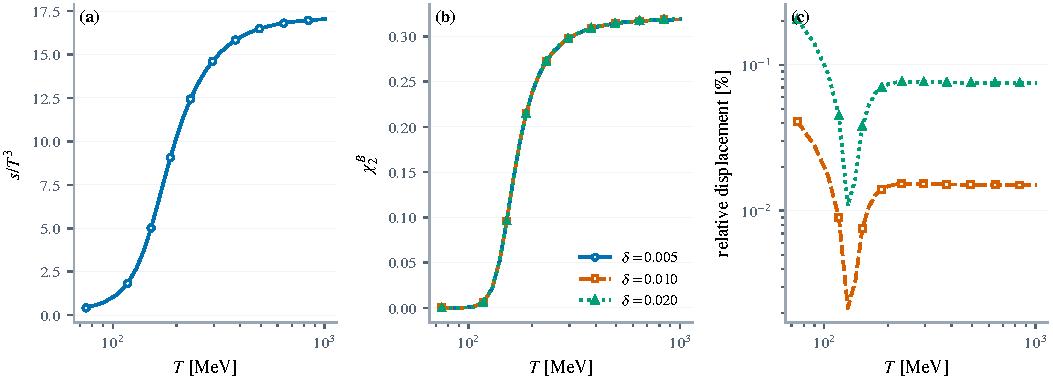
\includegraphics[width=\textwidth]{figures/thermodynamic_validation.pdf}
 \caption{Reproduction and numerical stability of neutral thermodynamics.
 Left: dimensionless entropy. Center: $\chi_2^B$ from the centered charge
 derivative in eq.~\eqref{eq:chi2fd}; the three step sizes are visually
 indistinguishable on this scale. Right: relative displacement from the
 finest-step result. This is a $\mu_B=0$ equilibrium validation and is not a
 finite-density CEP or spinodal claim.}
 \label{fig:thermodynamic-validation}
\end{figure}
\FloatBarrier

\section{Regular horizon expansion}
\label{app:horizon}

Writing
\begin{align}
 A&=A_1r+A_2r^2+\cdots,&h&=r+h_2r^2+\cdots,\nonumber\\
 \phi&=\phi_0+\phi_1r+\phi_2r^2+\cdots,&
 \Phi&=\Phi_1r+\Phi_2r^2+\cdots,
\end{align}
the compiled recurrence reproduces
\begin{align}
 A_1&=-\frac{2V_0+f_0\Phi_1^2}{6},&
 \phi_1&=V_{\phi,0}-\frac12f_{\phi,0}\Phi_1^2,\nonumber\\
 A_2&=-\frac{\phi_1^2}{12},&
 h_2&=\frac12(f_0\Phi_1^2-4A_1),\nonumber\\
 \Phi_2&=-\frac{\Phi_1}{2}\left(2A_1+\frac{f_{\phi,0}}{f_0}\phi_1\right).
\end{align}
Higher coefficients through fourth order are generated by truncated-series
arithmetic applied to the regular equations, rather than hand-entered formulas.

\section{Charged-hydrodynamic validation matrix}

With $w=\epsilon+P$, $n=\rhob$, and $\alpha=\mub/T$, the three longitudinal
hydrodynamic poles are compared to the roots of
\begin{equation}
 \det\begin{pmatrix}
 -\ii\omega&0&\ii kw\\
 \ii kP_\epsilon&\ii kP_n&-\ii\omega w+(\zeta+4\eta/3)k^2\\
 \sigma_BT k^2\alpha_\epsilon&-\ii\omega+\sigma_BT k^2\alpha_n&\ii kn
 \end{pmatrix}=0.
\end{equation}
Bulk viscosity, if required for this check, is imported from the existing PHA
transport calculation rather than presented as a new result.

\section{Validation and claim gates}
\label{app:gates}

The authoritative machine-readable spectrum stores the background horizon
data, physical thermodynamics, branch label, channel/helicity, momentum,
frequency, resolution, pencil and constraint residuals, condition number,
tracking parent, solver/backend metadata, compiler identity, commit, and
configuration hash. A mode enters a figure or table only after all relevant
acceptance fields pass. Coupled finite-momentum equations must also satisfy the
linearized Bianchi and Maxwell identities and reproduce the $k\to0$, neutral,
and conformal limits where available.

\bibliographystyle{JHEP}
\bibliography{references}

\end{document}
